\documentclass{beamer}
\graphicspath{ {./imagens/} }
\usetheme{Madrid}

\title{Simulação de termostato - Sistema CPS tempo misto (dinâmico e discreto)}
\author{Ricardo Rosal}
\begin{document}
\begin{frame}[plain]
    \maketitle
\end{frame}

\AtBeginSection[]{
	\begin{frame}
		\vfill
		\centering
		\begin{beamercolorbox}[sep=8pt,center,shadow=true,rounded=true]{title}
			\usebeamerfont{title}\insertsectionhead\par%
		\end{beamercolorbox}
		\vfill
	\end{frame}
}

\AtBeginSubsection[]{
	\begin{frame}
		\vfill
		\centering
		\begin{beamercolorbox}[sep=8pt,center,shadow=true,rounded=true]{title}
			\usebeamerfont{title}\insertsubsectionhead\par%
		\end{beamercolorbox}
		\vfill
	\end{frame}
}


\begin{frame}
	\tableofcontents
\end{frame}

\section{Sistemas Ciber-físicos}

\subsection{Definição}
\begin{frame}{O que é CPS?}
	\par \textbf{CPS (\emph{cyber-physical systems})} é uma técnica de modelagem de sistemas integrados que envolvem os componentes físicos e cibernéticos do mesmo.
	potencialmente interconectado em redes de sinais digitais altamente conectado.
	O componente \textbf{cibernético} do sistema corresponde ao modelo do comportamento lógico do sistema, comumente definido pelo método e algoritmo de controle.
	O componente \textbf{físico} corresponde o modelo do fenômeno natural, que é regido pelas leis da física.\cite{goebel_hybrid_2012}
	\begin{center}
		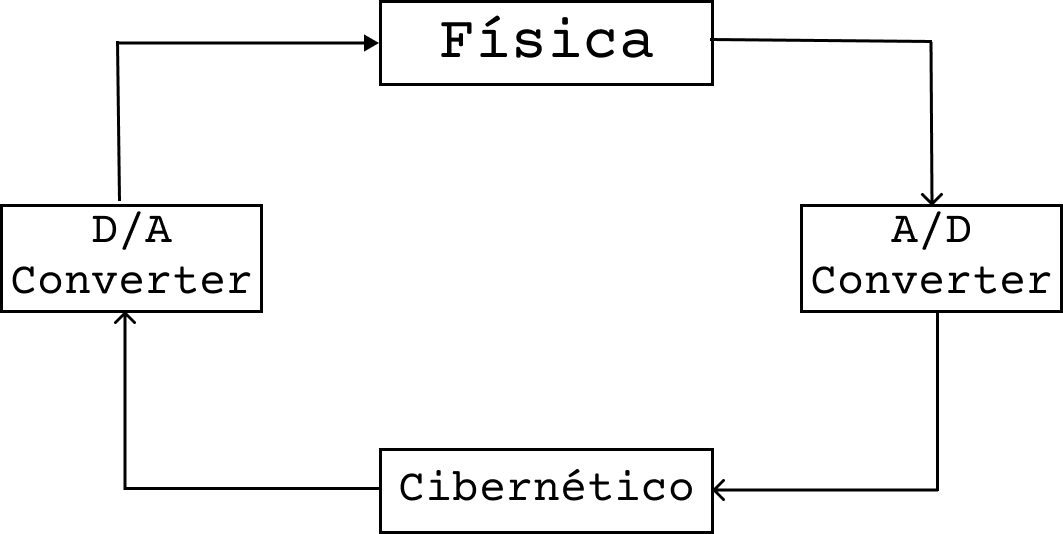
\includegraphics[width=0.5\textwidth]{imagens/CPS.png}
	\end{center}
\end{frame}

\subsection{Modelo de tempo discreto}
\begin{frame}{Modelo de tempo discreto}
	\begin{itemize}
		\item Um modelo de CPS de tempo discreto considera uma evolução discreta do tempo,
		o tempo evolui em passos periódicos e não continuo.
		\item A componente física do sistema, pela própria natureza do fenômeno natural costuma ser contínua,
		no entanto, nesses modelos devemos considerar a discretização da evolução do sistema físico no modelo.
		\item A modelagem matemática do componente físico de um modelo de CPS de tempo discreto normalmente são descritos por uma \textbf{equação de diferenças}, dada uma função $G(x,v)$ que descreve a evolução discreta do fenômeno físico, onde $x$ é o vetor de estado do sistema,  e $v$ é o vetor de entradas do sistema,
		que tem como saída a evolução discreta da medição do fenômeno no tempo.
		\item também uma função $\eta$ que descreve a saída do sistema.
	\end{itemize}
	
\end{frame}

\subsubsection{Modelo de equações de diferenças}

\begin{frame}{Modelo de tempo discreto}
	\begin{equation}
		x^{+}=G(x,v)
	\end{equation}
	\begin{equation}
		\eta^{+}=h(x,v)
	\end{equation}
	\par Para que seja possível calcular a solução dessa categoria de modelo, é necessário fornecer valores inicias do estado do fenômeno, definido pelo vetor $x$ e tambem as entradas do sistema cibernético $v$.
	Definidos respectivamente por $x_0$ e $v_0$.
	Definindo cada passo no tempo discreto como $k$, podemos reescrever o modelo discreto do CPS conforme abaixo.
	\begin{equation}
		x(k+1)=G(x(k),v(k))\;\forall\;k  \in \mathbb{N}
	\end{equation}
	\begin{equation}
		\eta(k+1)=h(x(k),v(k))\;\forall\;k  \in \mathbb{N}
	\end{equation}
	\par O Domínio das função $G(x,v)$ e $\eta(x,v)$, seu espaço é definido para todos os pontos possíveis pelo domínio dos sinais de entrada e do estado do sistema, $x$ e $v$.
\end{frame}

\subsection{modelo de tempo contínuo}

\begin{frame}{Modelo de tempo contínuo}
	\par Os modelos de tempo contínuo, como os de tempo discreto, também possuem uma componente física que recebe uma entrada $v$ e retorna uma saída $\eta$.
	A principal diferença é que essas funções variam no tempo contínuo, dado por $t \in \mathbb{R} \ge 0 := [0,+\infty)$ e não mais no tempo discreto, ou para ser mais preciso, na representação em eventos do tempo.
	\par Essa mudança implica na metodologia de descrição da dinâmica desses eventos, não podemos mais utilizar uma \textbf{equação de diferenças} para descrever a dinâmica, pois devemos descreve-la de forma contínua, e para isso será necessario o uso de algumas ferramentas do calculo, como as \textbf{equações diferenciais}.
	
	\begin{equation}
		\frac{dx}{dt}=F(x,v)
	\end{equation}
	\begin{equation}
		\eta = h(x,v)
	\end{equation}
	
	\par A solução desse sistema, é definida por uma função no tempo $x(t)$ que satisfaça a equação diferencial.
\end{frame}

\subsection{componente física do CPS}

\begin{frame}{Componente física do CPS - EDO ou EDP}
	\par A componente física de uma sistema CPS é definida por uma equação diferencial que define a dinâmica da variável física medida e controlada no sistema que vamos chamar aqui de $\dot{z}$ que é definida pela equação abaixo, onde $z$ é o estado atual do sistema e $\mu \in \mathbb{R}^{mp}$ é a entrada.
	\begin{equation}
		\dot{z} = F_p(z,\mu) \in \mathbb{R}^{np}
	\end{equation}
	
	\par E a saída do sistema, $y$, que é definida pela função abaixo.
	
	\begin{equation}
		y=h_p(z,\mu)\in \mathbb{R}^{hp}
	\end{equation}
	
	\par Onde o espaço dos sistema é definido pela seguinte restrição.
	\begin{equation}
		F_p:\mathbb{R}^{np} \times \mathbb{R}^{mp}
	\end{equation}
	\begin{equation}
		h_p:\mathbb{R}^{hp} \times \mathbb{R}^{mp}
	\end{equation}
\end{frame}

\subsection{componente cibernética do CPS}

\begin{frame}{Componente cibernética - FSM}	
	\begin{definition}[Maquina de Estados Finitos]
		Maquina de estados finitos é um método de modelagem de sistemas discretos que podem ser descritos por \textbf{estados} finitos e que a dinâmica possa ser descrita como uma \textbf{regra} de transição.
	\end{definition}
	
	\par As maquinas de estados finitos possui um número finito de estados definido pelo conjunto $Q$, e.g $\{A,B,C\} \in Q$, e um finito número de entradas $\Sigma$, e.g, $\{0,1\} \in \Sigma$.
	\par E a descrição da regra de transição de estados é da maquina de estado finito é definida pela função $\delta$, que tem como variável o estado atual do sistema $q$ e a entrada $v$.
	
	\begin{equation}
		q^{+}=\delta(q,v)
	\end{equation}
\end{frame}

\begin{frame}{Componente cibernética - FSM (Finite State Machine)}
	\par Um maquina de estados finitos deve conter os seguintes elementos:
	\begin{itemize}
		\item Um conjunto finito entrada $\Sigma$ da qual a entrada atual $v$ recebe seu valor;
		\item Um conjunto finito de estados $Q$ onde ocorre a dinâmica do estado $q$;
		\item Um conjunto de saída $\Delta$ onde a saida $\zeta$ recebe os valores;
		\item uma função de transição: $\delta: Q \times \Sigma \rightarrow \Delta$
	\end{itemize}
	\begin{center}
		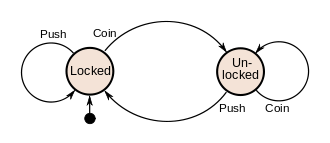
\includegraphics[width=0.5\textwidth]{imagens/fsm.png}
	\end{center}
\end{frame}

\begin{frame}{Conversor analógico digital}
	\par O conversor analógico-digital é um componente eletrônico, que precisa de uma memória para guardar informação convertida e precisará ser transmitida de por uma rede digital, essa memória será chamada aqui como $m_s$ e ela será reescrita a cada $\tau_s^{*}$.
	
	\begin{equation}
		\dot{m_s} = 0 \leftarrow m_s(t) = m_s(0)
	\end{equation}
	\begin{equation}
		m_s^{+} = v_s
	\end{equation}
	
	\par O ADC é definido por uma \textbf{equação diferencial} de duas variáveis e uma \textbf{equação de diferenças} de também duas variáveis.
	
	\begin{equation}
		\text{ADC contínuo} =
		\begin{cases}
			\dot{\tau_s} = 1\\
			\dot{m_s} = 0
		\end{cases}
		\text{quando $\tau_s \in [0,\tau_s^{*}]$}
	\end{equation}
	
	\begin{equation}
		\text{ADC discreto} =
		\begin{cases}
			\tau_s^{+} = 0\\
			m_s^{+} = v_s
		\end{cases}
		\text{quando $\tau_s = \tau_s^{*}$}
	\end{equation}
\end{frame}

\begin{frame}{Conversor digital analógico}
	\par no conversor digital analógica (DAC), o valor do estado da componente cibernetica do sistema é convertida para analógico para ser passado como entrada $v$ para a componente física do sistema, essa conversão é feita na periodicidade $\frac{1}{T_\eta}$, e muda de valor a cada $T_\eta$.
	
	\begin{equation}
		\text{DAC contínuo =}
		\begin{cases}
			\dot{m_{\eta}}=0\\
			\dot{\tau_{\eta}}=1
		\end{cases}
		\text{quando $\tau \in [0,T_{\eta}^{*})$}
	\end{equation}
	
	\begin{equation}
		\text{DAC discreto =}
		\begin{cases}
			m_{\eta}^{+}=v_{\eta}\\
			\tau_{\eta}^{+}=0
		\end{cases}
		\text{quando $\tau_\eta = T_\eta^{*}$}
	\end{equation}
\end{frame}

\section{Concepção}

\subsection{Modelo do Termostato - componente física}

\begin{frame}{Componente física - Termostato}
	\par Dado uma sala que possui uma temperatura que tem sua dinâmica definida pela função $T \in \mathbb{R}$ e um dispositivo que pode controlar essa temperatura, como um ar condicionado.
	Podemos modelar a componente física desse sistema pela seguinte equação diferencial.\cite{afroz_modeling_2018}
	\begin{equation}
		\dot{T} = (\alpha - \delta S) T + T_R
	\end{equation}
	\par Onde o parâmetro $\alpha$ é a taxa de troca de calor dado a carga térmica nesse espaço específico, o parâmetro $T_R$ é a taxa de influência da temperatura externa a essa sala e o $\delta$ é a capacidade de troca de calor do equipamento em questão, vezes o estado do próprio equipamento, onde estamos assumindo dois estados, ligado $(1)$ e desligado $(0)$.
\end{frame}

\begin{frame}{Componente física - Termostato}
	Convertendo esse modelo para a nossa convenção da componente física de um sistema CPS.
	\begin{equation}
		F_p(z,u) = (\alpha - \delta S)z + T_R
	\end{equation}
\end{frame}

\subsection{Modelo do Termostato - componente cibernética}

\begin{frame}{definição da maquina de estados finitos}
	\par Agora vamos definir o modelo de maquina de estados finito para um termostato, onde o conjunto de \textbf{estado} $Q$, é definido pelo modo de operação do termostato definido por: $q \in Q = \{ Ligado, Desligado\}$, conjunto do qual tambem é definido os valores da \textbf{saida} $\zeta$.
	\par A \textbf{entrada} é definido pelo variavel continua da temperatura, discretizada pelo conversor analógico digital, e limitado pelas restrições de temperatura maxima e mínima: $v \in \Sigma = T \in [ T_{min},T_{max}]$.
	\par E uma \textbf{função de transição} $\delta$ que define a regra para transição de estado da uma combinação de estado e entrada especifico.
	\begin{equation}
		\delta(v,q) =
		\begin{cases}
			ON & \text{$v \ge T^{max}$ e q=OFF}\\
			OFF & \text{$v \le T^{Min}$ e q=ON}
		\end{cases}
	\end{equation}
\end{frame}

\begin{frame}
e é definido tambem uma função de guarda que define as restrições da execução da maquina de estados finitos.
\begin{definition}
	A função de guarda $(l)$ define a combinação das variaveis do modelo da maquina de estado finito que ocorrerá as transições de estado.
\end{definition}

\begin{equation}
	l(v,q,\zeta) =
	\begin{cases}
		v \ge T_{max} & q^{+}=DESLIGADO\\
		v \le T_{min} & q^{+}=LIGADO
	\end{cases}       
\end{equation}

\begin{equation}
	\zeta = K(q) =
	\begin{cases}
		1 & \text{se q=ON}\\
		0 & \text{se q=OFF}
	\end{cases}
\end{equation}

\end{frame}

\begin{frame}
	\par Então, podemos definir completamentamente o modelo de maquina de estados definitos para controle de temperatura com um termostato pelo sistema de funções descritos abaixo.
	\begin{equation}
		\text{FSM com guarda} =
		\begin{cases}
			q^{+}=\delta(q,v)\\
			\zeta = K(q)\\
			l = l(q,v,\zeta)
		\end{cases}
	\end{equation}
\end{frame}

\begin{frame}{Componente Cibernética - Termostato}
		\par Componente Cibernética do modelo de CPS para o termostato, representado por uma maquina de estados finitos.
	\begin{figure}
		\centering
		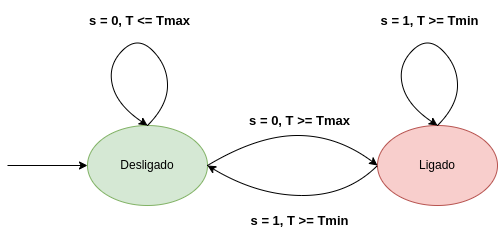
\includegraphics[width=.75\textwidth]{fsm_termostato.png}
		\caption{maquina de estados finitos do termostato}
		\label{fig:fsm}
	\end{figure}
\end{frame}

\section{Implementação}

\subsection{implementação da componente física}
\begin{frame}{Componente física}
	\begin{itemize}
		\item Foi criado uma função na linguagem de programação \textbf{Julia} que recebe um vetor de parâmetros do modelo e um vetor de variaveis para definir a equação diferencial ordinaria.
		\item Foi utilizado o pacote \textbf{DifferentialEquations.jl} para definir um objeto ODEProblem da biblioteca e resolver a equação diferencial numéricamente.
		\item O algoritmo númerico para solução da EDO escolhido foi o \textbf{Runge-Kutta de 5th ordem}.
	\end{itemize}
\end{frame}
\subsection{implementação da componente cibernetica}
\begin{frame}{Componente cibernética}
	\begin{itemize}
		\item foi criado uma função \textbf{callback} para ser executado a cada vez que a temperatura atingisse o valor maximo ou minino (implementação da função de guarda);
		\item essa função verificar o valor do \textbf{estado do termostato} (ligado ou desligado) e muda seu estado conforme o estado atual (implementação da função $\delta$);
		\item alem de mudar o termostato \textbf{ativa o estado para a componente física}, mudando a capacitância térmica do sistema.
	\end{itemize}
\end{frame}

\section{Análise}
\begin{frame}
	\begin{figure}
		\centering
		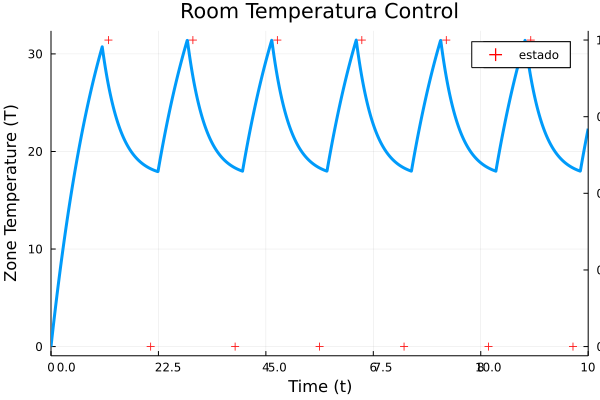
\includegraphics[width=.75\textwidth]{simulacao.png}
		\caption{simulaçao com com capacidade térmica 2x a carga térmica}
		\label{fig:simulacao}
	\end{figure}
\end{frame}

\begin{frame}
	\begin{figure}
		\centering
		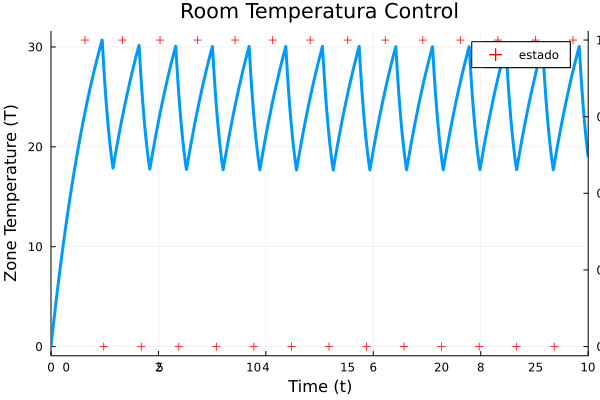
\includegraphics[width=.75\textwidth]{simulacao_4x.png}
		\caption{simulaçao com com capacidade térmica 4x a carga térmica}
		\label{fig:simulacao2}
	\end{figure}
\end{frame}

\begin{frame}{analise da simulação}
	\begin{itemize}
		\item Pode-se observar que quanto maior a capacidade do equipamento, mais rapido será o atingimento do setpoint de temperatura maxima e mínima, no entanto isso pode gerará mais eventos de partida e parada, o que pode diminuir a vida útil do mesmo.
		\item o modelo atual não leva em consideração ruidos nos sinais de carga térmica, como por exemplos novos equipamentos ligados no espaço ou numero maior de pessoas do que o esperado, isso pode ser simulado de forma estocástica a partir de uma distribuição de probabilidade e adicionar o parâmetro de carga térmica (fixo nesse modelo) como uma função que amostra de função inversa de uma distribuição de probabilidade.
	\end{itemize}
\end{frame}
\begin{frame}{Referências}
	\textbf{Referências:}
	\bibliographystyle{abbrv}
	\bibliography{ref.bib}
\end{frame}

\end{document}
